\textbf{Phần 1. Trắc nghiệm lựa chọn (Học sinh quan sát hình và chọn đáp án đúng)}
\setcounterpageref{ex}{0}

% --- CÂU 1 ---
\begin{ex} %[1D1N06]
Đoàn tàu chở các toa số từ $6$ đến $10$. Toa tàu đứng liền sau số $8$ mang số mấy?
\begin{center}
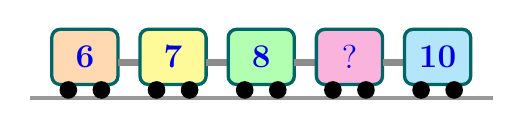
\begin{tikzpicture}[scale=0.7, baseline=(current bounding box.center)]
  \draw[line width=1.5pt, gray!80] (-4.2,-0.55) -- (4.2,-0.55);
  \foreach \i/\num/\cl in {0/6/orange!30, 1/7/yellow!40, 2/8/green!30, 3/{$\mathbf{?}$}/magenta!30, 4/10/cyan!30} {
    \draw[fill=\cl, draw=teal!80!black, line width=1.2pt, rounded corners=3pt] (-3.8+\i*1.6,-0.3) rectangle (-2.6+\i*1.6,0.7);
    \node[font=\large\bfseries, text=blue!90!black] at (-3.2+\i*1.6, 0.2) {\num};
    \fill[black] (-3.5+\i*1.6,-0.4) circle (0.16);
    \fill[black] (-2.9+\i*1.6,-0.4) circle (0.16);
    \ifnum\i<4
      \draw[line width=2.5pt, gray!90] (-2.6+\i*1.6,0.1) -- (-2.2+\i*1.6,0.1);
    \fi
  }
\end{tikzpicture}
\end{center}
\choice
{$7$}
{\True $9$}
{$10$}
{$6$}
\loigiai{
Thứ tự các số liên tiếp: $6, 7, 8, 9, 10$.\\
Số liền sau của số $8$ là số $9$.\\
\textbf{Đáp án của câu hỏi là B}
}
\end{ex}

% --- CÂU 2 ---
\begin{ex} %[1D1N06]
Quan sát bậc thang số: Bậc thang đứng liền trước số $5$ mang số mấy?
\begin{center}
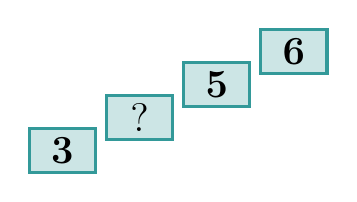
\begin{tikzpicture}[scale=0.7, baseline=(current bounding box.center)]
  \foreach \i/\num in {1/3, 2/{$\mathbf{?}$}, 3/5, 4/6} {
    \draw[fill=teal!20, draw=teal!80, line width=1.2pt] (\i*1.4, \i*0.6) rectangle (\i*1.4+1.2, \i*0.6+0.8);
    \node[font=\Large\bfseries] at (\i*1.4+0.6, \i*0.6+0.4) {\num};
  }
\end{tikzpicture}
\end{center}
\choice
{$3$}
{$6$}
{\True $4$}
{$7$}
\loigiai{
Số liền trước của số $5$ là số $4$.\\
\textbf{Đáp án của câu hỏi là C}
}
\end{ex}

% --- CÂU 3 ---
\begin{ex} %[1D1H06]
Đếm số chấm tròn ở hai bên và chọn dấu thích hợp điền vào ô tròn:
\begin{center}
\begin{tikzpicture}[scale=0.75, baseline=(current bounding box.center)]
  % 7 chấm cam bên trái
  \draw[fill=orange!10, draw=orange!60, line width=1pt] (-2.8,0) ellipse (1.8cm and 0.5cm);
  \foreach \x in {-3.8, -3.4, -3.0, -2.6, -2.2, -1.8, -2.8} { \fill[orange!90!black] (\x, 0.1) circle (0.18cm); }
  \node[font=\bfseries] at (-2.8, -0.8) {7 chấm};

  \draw[fill=yellow!25, draw=orange!80!black, line width=1.3pt] (0, 0.1) circle (0.45cm);
  \node[font=\Large\bfseries, text=red] at (0, 0.1) {?};

  % 9 chấm cam bên phải
  \draw[fill=orange!10, draw=orange!60, line width=1pt] (2.8,0) ellipse (2.0cm and 0.5cm);
  \foreach \x in {1.6, 2.0, 2.4, 2.8, 3.2, 3.6, 4.0, 2.2, 3.4} { \fill[orange!90!black] (\x, 0.1) circle (0.18cm); }
  \node[font=\bfseries] at (2.8, -0.8) {9 chấm};
\end{tikzpicture}
\end{center}
\choice
{\True $<$}
{$>$}
{$=$}
{Không có dấu}
\loigiai{
Vì $7 < 9$ nên điền dấu $<$.\\
\textbf{Đáp án của câu hỏi là A}
}
\end{ex}

% --- CÂU 4 ---
\begin{ex} %[1D1H06]
Quan sát sơ đồ gộp số: Gộp $4$ và $5$ được mấy?
\begin{center}
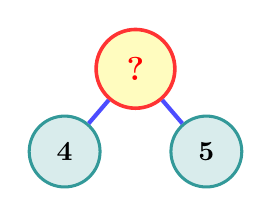
\begin{tikzpicture}[scale=0.75, baseline=(current bounding box.center)]
  \node[draw=red!80, fill=yellow!25, circle, line width=1.3pt, minimum size=1cm, font=\large\bfseries, text=red] (T) at (0,1.2) {?};
  \node[draw=teal!80, fill=teal!15, circle, line width=1.1pt, minimum size=0.9cm, font=\bfseries] (L) at (-1.2,-0.2) {4};
  \node[draw=teal!80, fill=teal!15, circle, line width=1.1pt, minimum size=0.9cm, font=\bfseries] (R) at (1.2,-0.2) {5};
  \draw[line width=1.5pt, blue!70] (T) -- (L);
  \draw[line width=1.5pt, blue!70] (T) -- (R);
\end{tikzpicture}
\end{center}
\choice
{$8$}
{$10$}
{$7$}
{\True $9$}
\loigiai{
Gộp $4$ và $5$ được $9$.\\
\textbf{Đáp án của câu hỏi là D}
}
\end{ex}

% --- CÂU 5 ---
\begin{ex} %[1D1H06]
Số $10$ gồm $6$ và mấy?
\begin{center}
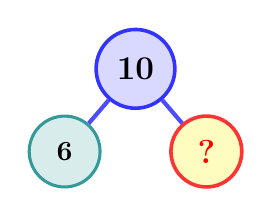
\begin{tikzpicture}[scale=0.75, baseline=(current bounding box.center)]
  \node[draw=blue!80, fill=blue!15, circle, line width=1.3pt, minimum size=1cm, font=\large\bfseries] (T) at (0,1.2) {10};
  \node[draw=teal!80, fill=teal!15, circle, line width=1.1pt, minimum size=0.9cm, font=\bfseries] (L) at (-1.2,-0.2) {6};
  \node[draw=red!80, fill=yellow!25, circle, line width=1.3pt, minimum size=0.9cm, font=\large\bfseries, text=red] (R) at (1.2,-0.2) {?};
  \draw[line width=1.5pt, blue!70] (T) -- (L);
  \draw[line width=1.5pt, blue!70] (T) -- (R);
\end{tikzpicture}
\end{center}
\choice
{$3$}
{$5$}
{\True $4$}
{$6$}
\loigiai{
$10$ gồm $6$ và $4$.\\
\textbf{Đáp án của câu hỏi là C}
}
\end{ex}

% --- CÂU 6 ---
\begin{ex} %[1D1H06]
Đếm số chú cá đang tung tăng bơi trong bình dưới đây:
\begin{center}
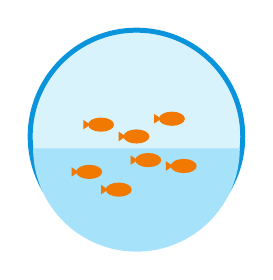
\begin{tikzpicture}[scale=0.75, baseline=(current bounding box.center)]
  \draw[fill=cyan!15, draw=cyan!80!blue, line width=1.8pt] (0,0) circle (1.8cm);
  \fill[cyan!35] (-1.75,-0.2) arc (180:360:1.75cm) -- cycle;
  \foreach \px/\py in {-0.8/-0.6, -0.3/-0.9, -0.6/0.2, 0.2/-0.4, 0.6/0.3, 0.8/-0.5, 0.0/0.0} {
    \fill[orange!95!black] (\px,\py) ellipse (0.22cm and 0.12cm);
    \fill[orange!95!black] (\px-0.18,\py) -- (\px-0.3,\py+0.08) -- (\px-0.3,\py-0.08) -- cycle;
  }
\end{tikzpicture}
\end{center}
\choice
{$6$ chú cá}
{$8$ chú cá}
{$5$ chú cá}
{\True $7$ chú cá}
\loigiai{
Đếm trong bình có đúng $7$ chú cá đang bơi.\\
\textbf{Đáp án của câu hỏi là D}
}
\end{ex}

% --- CÂU 7 ---
\begin{ex} %[1D1V06]
Trong các ngôi sao mang số $2, 9, 5, 0$, ngôi sao nào mang số \textbf{lớn nhất}?
\begin{center}
\begin{tikzpicture}[scale=0.75, baseline=(current bounding box.center)]
  \foreach \x/\num in {-2.7/2, -0.9/9, 0.9/5, 2.7/0} {
    \node[draw=orange!80!black, fill=yellow!80, star, star points=5, star point ratio=2.2, line width=1.1pt, minimum size=1.1cm] at (\x,0) {};
    \node[font=\bfseries\normalsize, text=red!85!black] at (\x,-0.02) {\num};
  }
\end{tikzpicture}
\end{center}
\choice
{\True $9$}
{$5$}
{$2$}
{$0$}
\loigiai{
So sánh các số: $9 > 5 > 2 > 0$. Số lớn nhất là số $9$.\\
\textbf{Đáp án của câu hỏi là A}
}
\end{ex}

% --- CÂU 8 ---
\begin{ex} %[1D1V06]
Trong chùm bóng bay mang số $8, 3, 10, 6$, quả bóng nào mang số \textbf{bé nhất}?
\begin{center}
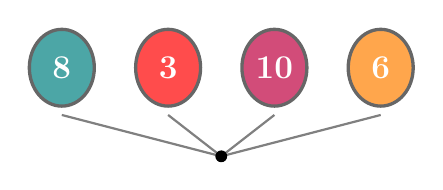
\begin{tikzpicture}[scale=0.75, baseline=(current bounding box.center)]
  \foreach \x/\num/\c in {-2.7/8/teal, -0.9/3/red, 0.9/10/purple, 2.7/6/orange} {
    \draw[line width=0.8pt, gray] (\x,-0.8) -- (0,-1.5);
    \draw[fill=\c!70, draw=black!60, line width=1.2pt] (\x,0) ellipse (0.55cm and 0.65cm);
    \node[font=\large\bfseries, text=white] at (\x,0) {\num};
  }
  \fill[black] (0,-1.5) circle (0.1cm);
\end{tikzpicture}
\end{center}
\choice
{$8$}
{\True $3$}
{$6$}
{$10$}
\loigiai{
So sánh: $3 < 6 < 8 < 10$. Số bé nhất là số $3$.\\
\textbf{Đáp án của câu hỏi là B}
}
\end{ex}

% --- CÂU 9 ---
\begin{ex} %[1D1V06]
Sắp xếp các số $0, 5, 2, 8$ theo thứ tự từ \textbf{bé đến lớn}:
\begin{center}
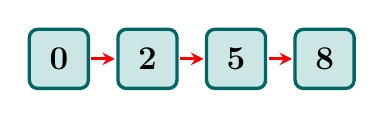
\begin{tikzpicture}[scale=0.75, baseline=(current bounding box.center)]
  \foreach \i/\num in {0/0, 1/2, 2/5, 3/8} {
    \draw[fill=teal!20, draw=teal!80!black, line width=1.2pt, rounded corners=3pt] (\i*1.5,-0.4) rectangle (\i*1.5+1.0,0.6);
    \node[font=\large\bfseries] at (\i*1.5+0.5, 0.1) {\num};
    \ifnum\i<3
      \draw[->, >=stealth, line width=1pt, red] (\i*1.5+1.05,0.1) -- (\i*1.5+1.45,0.1);
    \fi
  }
\end{tikzpicture}
\end{center}
\choice
{$8, 5, 2, 0$}
{$0, 5, 2, 8$}
{$2, 0, 5, 8$}
{\True $0, 2, 5, 8$}
\loigiai{
Từ bé đến lớn: $0 < 2 < 5 < 8$.\\
\textbf{Đáp án của câu hỏi là D}
}
\end{ex}

% --- CÂU 10 ---
\begin{ex} %[1D1V06]
Tìm số thích hợp điền vào ô trống: $7 < \mathbf{?} < 9$.
\begin{center}
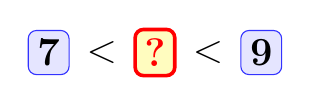
\begin{tikzpicture}[scale=0.75, baseline=(current bounding box.center)]
  \node[draw=blue!80, fill=blue!10, rounded corners=3pt, font=\Large\bfseries] at (-1.8,0) {7};
  \node[font=\Large\bfseries] at (-0.9,0) {$<$};
  \node[draw=red, fill=yellow!25, line width=1.3pt, rounded corners=3pt, font=\Large\bfseries, text=red] at (0,0) {?};
  \node[font=\Large\bfseries] at (0.9,0) {$<$};
  \node[draw=blue!80, fill=blue!10, rounded corners=3pt, font=\Large\bfseries] at (1.8,0) {9};
\end{tikzpicture}
\end{center}
\choice
{$7$}
{$9$}
{\True $8$}
{$10$}
\loigiai{
Số ở giữa 7 và 9 là số $8$ ($7 < 8 < 9$).\\
\textbf{Đáp án của câu hỏi là C}
}
\end{ex}

% --- CÂU 11 ---
\begin{ex} %[1D1V06]
Đĩa A có $6$ quả táo, đĩa B có $6$ quả lê:
\begin{center}
\begin{tikzpicture}[scale=0.75, baseline=(current bounding box.center)]
  \draw[fill=red!10, draw=red!70, line width=1.2pt] (-2,0) ellipse (1.6cm and 0.5cm);
  \node[font=\small\bfseries] at (-2,0) {Đĩa A: 6 quả};
  \draw[fill=green!10, draw=green!70, line width=1.2pt] (2,0) ellipse (1.6cm and 0.5cm);
  \node[font=\small\bfseries] at (2,0) {Đĩa B: 6 quả};
\end{tikzpicture}
\end{center}
Khẳng định nào sau đây đúng?
\choice
{Đĩa A nhiều hơn đĩa B}
{\True Số quả ở hai đĩa bằng nhau}
{Đĩa B nhiều hơn đĩa A}
{Không so sánh được}
\loigiai{
Vì cả hai đĩa đều có $6$ quả nên số quả ở hai đĩa bằng nhau ($6 = 6$).\\
\textbf{Đáp án của câu hỏi là B}
}
\end{ex}

% --- CÂU 12 ---
\begin{ex} %[1D1C06]
Đếm lùi trên thân chú sâu: $10, 9, \mathbf{?}, 7, 6$. Đốt thân có dấu $\mathbf{?}$ mang số mấy?
\begin{center}
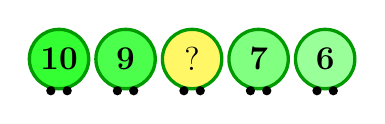
\begin{tikzpicture}[scale=0.65, baseline=(current bounding box.center)]
  \foreach \x/\num/\c in {0/10/green!80, 1.3/9/green!70, 2.6/{$\mathbf{?}$}/yellow!60, 3.9/7/green!50, 5.2/6/green!40} {
    \draw[fill=\c, draw=green!60!black, line width=1.2pt] (\x,0) circle (0.58cm);
    \node[font=\large\bfseries, text=black] at (\x,0) {\num};
    \fill[black] (\x-0.16,-0.62) circle (0.09); \fill[black] (\x+0.16,-0.62) circle (0.09);
  }
\end{tikzpicture}
\end{center}
\choice
{\True $8$}
{$9$}
{$7$}
{$6$}
\loigiai{
Đếm lùi: $10, 9, 8, 7, 6$. Số còn thiếu là số $8$.\\
\textbf{Đáp án của câu hỏi là A}
}
\end{ex}

% =========================================================================
% PHẦN 2: TRẮC NGHIỆM ĐÚNG SAI (QUAN SÁT TRANH MINH HỌA)
% =========================================================================
\textbf{Phần 2. Trắc nghiệm đúng sai (Xét tính đúng/sai của các nhận định)}
\setcounterpageref{ex}{0}

% --- CÂU 13 ---
\begin{ex} %[1D1H06]
Cho nhóm các số: $0, 4, 7, 10$. Xét tính đúng sai của các câu sau:
\choiceTF
{\True Số bé nhất trong nhóm là số $0$.}
{\True Số lớn nhất trong nhóm là số $10$.}
{Số $4$ lớn hơn số $7$.}
{\True Số $7$ bé hơn số $10$.}
\loigiai{
\begin{itemize}
    \item Bé nhất là $0$: \textbf{Đúng}.
    \item Lớn nhất là $10$: \textbf{Đúng}.
    \item $4 < 7$ (nói $4 > 7$ là sai): \textbf{Sai}.
    \item $7 < 10$: \textbf{Đúng}.
\end{itemize}
}
\end{ex}

% --- CÂU 14 ---
\begin{ex} %[1D1V06]
Xét tính đúng sai của các cách tách gộp số dưới đây:
\choiceTF
{\True Số $10$ gồm $5$ và $5$.}
{\True Gộp $3$ và $6$ được $9$.}
{Số $9$ gồm $4$ và $6$.}
{\True Gộp $2$ và $5$ được $7$.}
\loigiai{
\begin{itemize}
    \item $10$ gồm $5$ và $5$: \textbf{Đúng}.
    \item Gộp $3$ và $6$ được $9$: \textbf{Đúng}.
    \item $9$ gồm $4$ và $5$ (nói $6$ là sai vì $4+6=10$): \textbf{Sai}.
    \item Gộp $2$ và $5$ được $7$: \textbf{Đúng}.
\end{itemize}
}
\end{ex}

% =========================================================================
% PHẦN 3: TRẢ LỜI NGẮN (ĐIỀN SỐ THÍCH HỢP VÀO Ô TRỐNG)
% =========================================================================
\textbf{Phần 3. Trả lời ngắn (Quan sát hình vẽ và điền số thích hợp)}
\setcounterpageref{ex}{0}

% --- CÂU 15 ---
\begin{ex} %[1D1H06]
Đếm số chấm tròn trong khung dưới đây:
\begin{center}
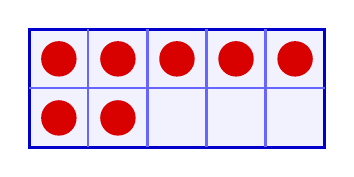
\begin{tikzpicture}[scale=0.75, baseline=(current bounding box.center)]
  \draw[line width=1.2pt, blue!80!black, fill=blue!5] (0,0) rectangle (5,2);
  \draw[line width=0.8pt, blue!60] (0,1) -- (5,1);
  \foreach \x in {1,2,3,4} { \draw[line width=0.8pt, blue!60] (\x,0) -- (\x,2); }
  % 7 chấm tròn đỏ (hàng trên 5, hàng dưới 2)
  \foreach \x in {0.5, 1.5, 2.5, 3.5, 4.5} { \fill[red!85!black] (\x, 1.5) circle (0.3cm); }
  \foreach \x in {0.5, 1.5} { \fill[red!85!black] (\x, 0.5) circle (0.3cm); }
\end{tikzpicture}
\end{center}
\shortans{7}
\loigiai{
\textbf{Đáp số:} $7$\\
Đếm trong khung có $7$ chấm tròn.
}
\end{ex}

% --- CÂU 16 ---
\begin{ex} %[1D1H06]
Tìm số liền sau của số $9$.
\shortans{10}
\loigiai{
\textbf{Đáp số:} $10$\\
Số liền sau của số $9$ là số $10$.
}
\end{ex}

% --- CÂU 17 ---
\begin{ex} %[1D1V06]
Tìm số liền trước của số $7$.
\shortans{6}
\loigiai{
\textbf{Đáp số:} $6$\\
Số liền trước của số $7$ là số $6$.
}
\end{ex}

% --- CÂU 18 ---
\begin{ex} %[1D1V06]
Gộp $4$ và $3$ được mấy?
\shortans{7}
\loigiai{
\textbf{Đáp số:} $7$\\
Gộp $4$ và $3$ được $7$.
}
\end{ex}

% --- CÂU 19 ---
\begin{ex} %[1D1V06]
Số $9$ gồm $5$ và mấy?
\shortans{4}
\loigiai{
\textbf{Đáp số:} $4$\\
$9$ gồm $5$ và $4$.
}
\end{ex}

% --- CÂU 20 ---
\begin{ex} %[1D1C06]
Tìm số thích hợp điền vào ô trống: $8 < \dots < 10$.
\shortans{9}
\loigiai{
\textbf{Đáp số:} $9$\\
Số ở giữa 8 và 10 là số $9$.
}
\end{ex}
